\documentclass[11pt,a4paper]{article}
\usepackage[margin=19mm]{geometry}
\usepackage[T1]{fontenc}
\usepackage{lmodern}
\usepackage{microtype}
\usepackage{amsmath}
\usepackage{amssymb}
\usepackage{xcolor}
\usepackage{tikz}
\usetikzlibrary{arrows.meta,shapes.geometric,calc}
\usepackage[hidelinks]{hyperref}

\definecolor{ink}{HTML}{243746}
\definecolor{bluewash}{HTML}{EDF4FA}
\definecolor{blueedge}{HTML}{607F99}
\definecolor{greenwash}{HTML}{EAF4ED}
\definecolor{greenedge}{HTML}{62856C}
\definecolor{rosewash}{HTML}{FAEEEE}
\definecolor{roseedge}{HTML}{A17777}

\pagestyle{plain}
\setlength{\parindent}{0pt}
\setlength{\parskip}{7pt}
\color{ink}

\newcommand{\SE}[2]{\ensuremath{#1\text{-}\mathrm{SE}_{#2}}}
\tikzset{
    flow/.style={->,draw=ink},
    box/.style={rectangle,rounded corners=3pt,draw=blueedge,
        fill=bluewash,align=center,text width=4.7cm,
        minimum height=0.9cm,inner sep=6pt},
    decision/.style={diamond,aspect=2.7,draw=blueedge,
        fill=bluewash,align=center,text width=3.2cm,inner sep=3pt},
    action/.style={box,text width=2.5cm,minimum height=1.05cm},
    accept/.style={box,draw=greenedge,fill=greenwash,text width=2.8cm},
    reject/.style={box,draw=roseedge,fill=rosewash,text width=2.9cm}
}

% One spacious primary-stage panel per page.
% Arguments: basis, opposite basis, circuit label, table, zero-flag continuation,
% flagged-correction continuation.
\newcommand{\PrimaryPanel}[6]{%
\begin{tikzpicture}[>=Latex,font=\small,line width=0.8pt,
    branch/.style={box,text width=4.7cm,minimum height=1.5cm}]
    \node[box] (read) at (0,0)
        {Run \SE{#1}{#3}\\Read $f_{#1},\sigma_{#1}$};
    \node[decision,text width=1.45cm,aspect=2.5] (zero) at (0,-2.3)
        {$f_{#1}=0$?};
    \node[decision,text width=2.3cm,aspect=2.3] (decode) at (-4.4,-5.0)
        {Correctable\\$\sigma_{#1}$?};
    \node[box,text width=4.7cm,minimum height=1.3cm] (lookup) at (3.25,-5.0)
        {Select the flagged action\\$#4$};
    \node[accept,text width=3.8cm,minimum height=1.5cm] (clean) at (-4.4,-9.0)
        {$\mathsf C$: correct now\\Apply $C_{#1}$\\#5};
    \node[reject,text width=3.8cm,minimum height=1.3cm] (bad) at (-4.4,-14.0)
        {$\mathsf D$: discard\\Stop};
    \node[branch,draw=greenedge,fill=greenwash,minimum height=1.9cm]
        (correct) at (3.25,-8.4)
        {$\mathsf C$: correct now\\Apply $C_{#1}$\\#6};
    \node[branch] (nonft) at (3.25,-11.3)
        {$\mathsf N$: non-FT follow-up\\Run \SE{#2}{1}\\Then use Figure 2};
    \node[branch] (ft) at (3.25,-14.2)
        {$\mathsf F$: 1-FT follow-up\\Run \SE{#2}{2}\\Then use Figure 2};
    \node[branch,draw=roseedge,fill=rosewash] (discard) at (3.25,-17.1)
        {$\mathsf D$: discard\\Stop};
    \draw[flow] (read) -- (zero);
    \draw[flow] (zero.west) -| node[pos=0.25,above]{Yes} (decode.north);
    \draw[flow] (zero.east) -| node[pos=0.25,above]{No} (lookup.north);
    \draw[flow] (decode.south) -- node[right]{Yes} (clean.north);
    \draw[flow] (decode.west) -- (-7.4,-5.0)
        node[midway,above]{No} -- (-7.4,-14.0) -- (bad.west);
    \draw[draw=ink] (lookup.south) -- (3.25,-6.35) -- (0,-6.35) -- (0,-17.1);
    \draw[flow] (0,-8.4) -- (correct.west);
    \draw[flow] (0,-11.3) -- (nonft.west);
    \draw[flow] (0,-14.2) -- (ft.west);
    \draw[flow] (0,-17.1) -- (discard.west);
\end{tikzpicture}%
}

\begin{document}

{\LARGE\bfseries Minimal adaptive Steane EC}\par
{\large Fault-tolerance conditions and the complete control flow}

\textbf{1. Gottesman's original EC properties.}
The original presentation uses an $[[n,1,2t+1]]$ code, ordinary Pauli weight,
and an EC gadget with no discard outcome [1, Definitions 1 and 5].
Here $r$ counts incoming errors and $s$ counts faulty circuit locations.

For code space $\mathcal Q$, let $P_r$ project onto
\[
 \operatorname{span}\{E|\psi\rangle:\ |\psi\rangle\in\mathcal Q,
                    \ \operatorname{wt}(E)\leq r\},
 \qquad \mathcal F_r(\rho)=P_r\rho P_r.
\]
Weight counts nonidentity tensor factors. The ideal decoder $\mathcal D$
performs error correction and decoding with no faults. For every EC
implementation $\mathcal E_F$ containing $s$ faulty locations:
\begin{align}
 \mathcal F_s\circ\mathcal E_F&=\mathcal E_F
       &&\text{if }s\leq t, \tag{EC A}\label{eq:eca}\\
 \mathcal D\circ\mathcal E_F\circ\mathcal F_r
       &=\mathcal D\circ\mathcal F_r
       &&\text{if }r+s\leq t. \tag{EC B}\label{eq:ecb}
\end{align}
EC A applies to arbitrary inputs: output errors are bounded relative to
\emph{some} codeword. EC B preserves the incoming ideal-decoded logical state.

\textbf{2. Even distance.}
For $d=2m$, the correction radius is $t=m-1$.
The original conditions apply unchanged:
\[
 \text{EC A: }s\leq m-1,
 \qquad
 \text{EC B: }r+s\leq m-1.
\]
For $d=4$, these bounds are $s\leq1$ and $r+s\leq1$.
Even distance does not itself extend the logical guarantee to two faults.
For $k>1$, the decoder outputs all $k$ logical qubits and EC B must preserve
their joint state.

\textbf{3. The CSS, postselected contract proposed here.}
These are explicit modifications of the original definition.
Replace the filter by the projector $P_r^{\mathrm{CSS}}$ onto
\[
 \operatorname{span}\{X(x)Z(z)|\psi\rangle:\ |\psi\rangle\in\mathcal Q,
         \ \operatorname{wt}(x)\leq r,\ \operatorname{wt}(z)\leq r\}.
\]
Thus $X_iZ_j$ with $i\ne j$ passes the CSS one-error filter [2].
Use an ideal decoder that corrects this CSS error set.
Writing $\mathcal E_F^{\mathrm{acc}}$ for the unnormalized accepted-output map,
require
\begin{align*}
 \mathcal F_s^{\mathrm{CSS}}\circ\mathcal E_F^{\mathrm{acc}}
     &=\mathcal E_F^{\mathrm{acc}} &&(s\leq t),\\
 \mathcal D\circ\mathcal E_F^{\mathrm{acc}}\circ\mathcal F_r^{\mathrm{CSS}}
     &=\mathcal D\circ\mathcal F_r^{\mathrm{CSS}} &&(r+s\leq t).
\end{align*}
The second equality requires both acceptance and logical preservation.
Outside that regime, rejection is permitted.

\textbf{Additional even-distance check.}
We propose also checking bounded histories with $r+s\leq m$ and requiring
accepted outputs to pass the CSS $s$-filter. In particular, two internal
faults at $d=4$ may leave two errors per component.
This extra output bound is a design choice; it does not guarantee logical
correctness at order $m$.

{\footnotesize
[1] D.~Gottesman,
\href{https://arxiv.org/pdf/0904.2557}{\emph{An Introduction to Quantum Error
Correction and Fault-Tolerant Quantum Computation}}, Sec.~4.2, pp.~19--22.
\quad [2] D.~Gottesman,
\href{https://www2.perimeterinstitute.ca/personal/dgottesman/QECC2007/Sols6.pdf}{\emph{Solution Set 6}}, Problem~2.
}

\clearpage
{\LARGE\bfseries The $d=4$ cycle: start with Z-SE}\par
\textbf{Follow-up notation:}
non-FT follow-up $=\mathrm{SE}_1$;
1-FT follow-up $=\mathrm{SE}_2$.
The basis is specified separately as X or Z.

Write $f_Z,\sigma_Z$ for the Z-extraction flags and syndrome, and
$f_X,\sigma_X$ for the X-extraction readouts. Subscripts name the measured
stabilizers: Z-SE diagnoses X errors, and X-SE diagnoses Z errors.

\begin{center}
\PrimaryPanel{Z}{X}{4}{\mathcal A_Z(f_Z,\sigma_Z)}
    {Next: \SE{X}{4} (Figure 1b)}
    {$b_{\min}=1$: next \SE{X}{2}\\$b_{\min}=2$: next \SE{X}{1}}

{\small\textbf{Figure 1a.} First split on $f_Z=0$; only the flagged arm offers follow-up SE.}
\end{center}

The flagged-arm continuations shown are candidates, enabled only after
verification. $b_{\min}$ is the least number of internal faults compatible
with the observations. A correction does not reset this fault count.

\clearpage
{\LARGE\bfseries The $d=4$ cycle: the X stage}\par
The previous branch selects $\delta$: the unflagged Z path uses $\delta=4$;
a flagged Z path can use $\delta=2$ or $1$ when certified.
The earlier Z readouts remain explicit inputs to the X-stage table.

\begin{center}
\PrimaryPanel{X}{Z}{\delta}{\mathcal A_X(f_Z,\sigma_Z;f_X,\sigma_X)}
    {Accept}
    {Accept}

{\small\textbf{Figure 1b.} The same split and four flagged actions apply at the X stage.}
\end{center}

For both primaries: zero flags plus a correctable syndrome means correct now;
zero flags plus an uncorrectable syndrome means discard.
Here ``correctable'' is determined by the verified stage decoder, using the
readouts already available. A zero syndrome permits the identity correction.

\clearpage
{\LARGE\bfseries Every adaptive follow-up: the same split}\par
For a follow-up in basis $B$, first test the current $f_B$.
Repeated readouts use superscripts, such as $f_X^{(1)},\sigma_X^{(1)}$.
The bold symbols below collect those explicit readouts by basis; there is no
opaque history variable.

\begin{center}
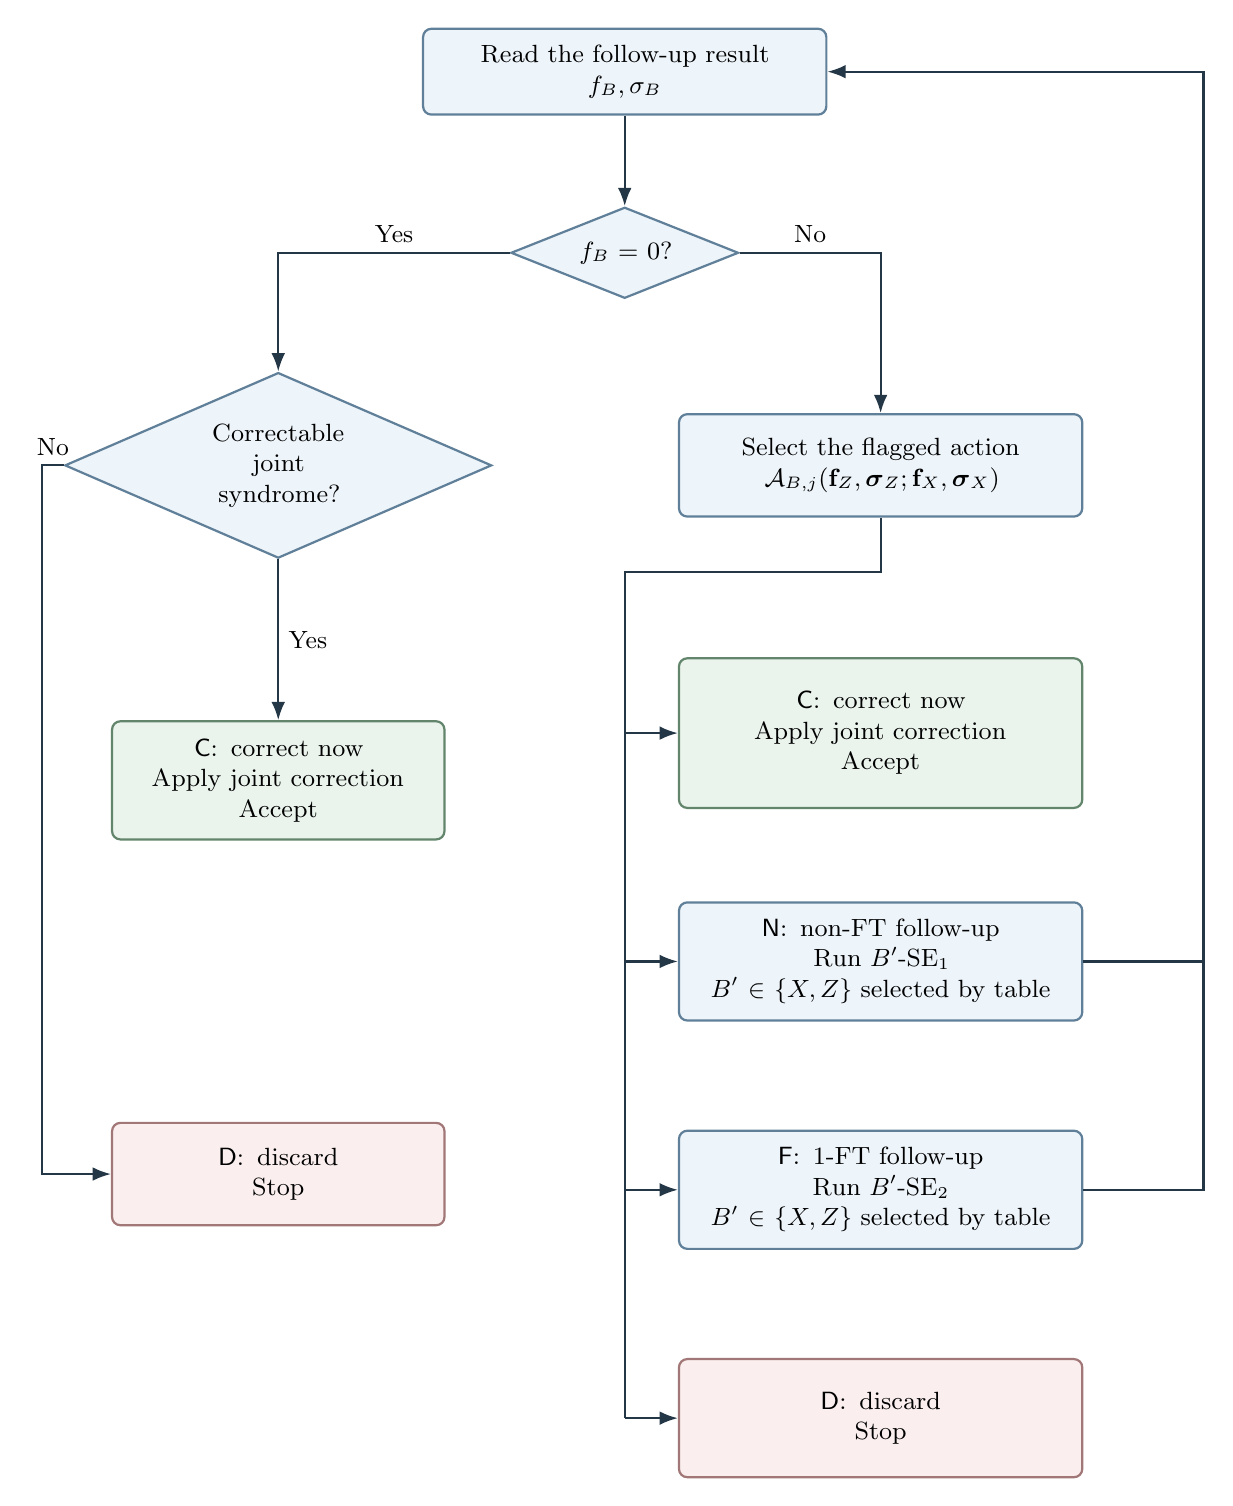
\begin{tikzpicture}[>=Latex,font=\small,line width=0.8pt,
    branch/.style={box,text width=4.7cm,minimum height=1.5cm}]
    \node[box] (read) at (0,0)
        {Read the follow-up result\\$f_B,\sigma_B$};
    \node[decision,text width=1.45cm,aspect=2.5] (zero) at (0,-2.3)
        {$f_B=0$?};
    \node[decision,text width=2.3cm,aspect=2.3] (decode) at (-4.4,-5.0)
        {Correctable joint\\syndrome?};
    \node[box,text width=4.7cm,minimum height=1.3cm] (lookup) at (3.25,-5.0)
        {Select the flagged action\\
         $\mathcal A_{B,j}(\mathbf f_Z,\boldsymbol\sigma_Z;
                          \mathbf f_X,\boldsymbol\sigma_X)$};
    \node[accept,text width=3.8cm,minimum height=1.5cm] (clean) at (-4.4,-9.0)
        {$\mathsf C$: correct now\\Apply joint correction\\Accept};
    \node[reject,text width=3.8cm,minimum height=1.3cm] (bad) at (-4.4,-14.0)
        {$\mathsf D$: discard\\Stop};
    \node[branch,draw=greenedge,fill=greenwash,minimum height=1.9cm]
        (correct) at (3.25,-8.4)
        {$\mathsf C$: correct now\\Apply joint correction\\Accept};
    \node[branch] (nonft) at (3.25,-11.3)
        {$\mathsf N$: non-FT follow-up\\Run \SE{B'}{1}\\$B'\in\{X,Z\}$ selected by table};
    \node[branch] (ft) at (3.25,-14.2)
        {$\mathsf F$: 1-FT follow-up\\Run \SE{B'}{2}\\$B'\in\{X,Z\}$ selected by table};
    \node[branch,draw=roseedge,fill=rosewash] (discard) at (3.25,-17.1)
        {$\mathsf D$: discard\\Stop};
    \draw[flow] (read) -- (zero);
    \draw[flow] (zero.west) -| node[pos=0.25,above]{Yes} (decode.north);
    \draw[flow] (zero.east) -| node[pos=0.25,above]{No} (lookup.north);
    \draw[flow] (decode.south) -- node[right]{Yes} (clean.north);
    \draw[flow] (decode.west) -- (-7.4,-5.0)
        node[midway,above]{No} -- (-7.4,-14.0) -- (bad.west);
    \draw[draw=ink] (lookup.south) -- (3.25,-6.35) -- (0,-6.35) -- (0,-17.1);
    \draw[flow] (0,-8.4) -- (correct.west);
    \draw[flow] (0,-11.3) -- (nonft.west);
    \draw[flow] (0,-14.2) -- (ft.west);
    \draw[flow] (0,-17.1) -- (discard.west);
    \draw[draw=ink] (nonft.east) -- (7.35,-11.3);
    \draw[flow] (ft.east) -- (7.35,-14.2) -- (7.35,0) -- (read.east);
\end{tikzpicture}

{\small\textbf{Figure 2.} Both follow-up circuits return to the same explicit dispatcher.}
\end{center}

For general distance $d$, start with \SE{Z}{d}; the zero-flag correction path
continues with \SE{X}{d}. The labels non-FT and 1-FT always mean
$\mathrm{SE}_1$ and $\mathrm{SE}_2$, respectively.
Other protection levels must be named by their explicit circuit label
$\mathrm{SE}_{\delta}$ and verified separately.
The data-code distance stays $d$ throughout.

\clearpage
{\LARGE\bfseries What the finer flag split buys us}\par

\textbf{A flag spends fault budget.}
For all six saved extraction gadgets, ideal extraction gives zero flags for
\emph{every} incoming data Pauli. A nonzero flag therefore certifies a new
internal fault in that extraction. Zero flags do not certify zero faults.
This interpretation relies on the verified circuit response, not on counting
how many flag bits are one [3].

In the additional two-fault analysis for $d=4$:
\begin{center}
\begin{tabular}{@{}p{3.1cm}p{5.4cm}p{7.0cm}@{}}
\textbf{Certified minimum} & \textbf{Remaining new faults} & \textbf{Candidate next X-SE}\\[4pt]
$b_{\min}=0$ & At most two & Keep the clean \SE{X}{4} path.\\[4pt]
$b_{\min}=1$ & At most one & Consider 1-FT \SE{X}{2}.\\[4pt]
$b_{\min}=2$ & None within this budget & Consider non-FT \SE{X}{1}.\\
\end{tabular}
\end{center}
These are candidate protection levels, not automatic action assignments.
Correction and discard remain available in the flagged arm.
For general fault-analysis order $q$, the analogous upper bound on further
internal faults is $q-b_{\min}$; complete branch verification still decides
which circuit is sufficient.

\textbf{Use the specific pattern, then the syndrome.}
On the saved Z-primary circuit, printed flag patterns
\texttt{00000011011} and \texttt{00000011100} have minimum internal fault
orders one and two, respectively. Thus the test $f_Z\ne0$ is a useful first
split, but is too coarse to choose the minimal follow-up on its own.

\textbf{Do not silently forget earlier readouts.}
For primary flag mask $1$, the exact checks found safe joint corrections for
all 4,096 unflagged observed prefixes after either \SE{X}{1} or \SE{X}{2},
when $\sigma_Z$ was retained. Merging by the latest $f_X,\sigma_X$ alone
lost required corrections in two groups. A branch-specific table can encode
older readouts without a generic $h$ parameter; dropping them needs a proof.
These counts describe observed prefixes, not probabilities.

\textbf{Why d2 is not always necessary.}
The current contract is deliberately weak at two internal faults: for this
code, every syndrome passes the CSS two-error filter (64 component syndromes
in each basis). It does not force logical correctness at that order.
Consequently, even a one-fault-compatible primary flag can sometimes admit d1.
The check above establishes this for one primary flag pattern only, with the
current gate/reset/measurement fault model and no implicit idle faults.
It does not certify the complete policy or its logical error rate.

\textbf{Rules fixed by this proposal.}
Every stage uses the explicit zero/nonzero split. The planner must reject
any table that sends a guaranteed-acceptance history to discard.
All subsequent faults, including physical correction faults, count toward
the same budget. Tables are minimized over complete continuations and must
still be synthesized and verified for the supplied circuits.

{\footnotesize
[3] R.~Chao and B.~W.~Reichardt,
\href{https://arxiv.org/abs/1912.09549}{\emph{Flag fault-tolerant error correction
for any stabilizer code}}, Sec.~II.
The circuit-specific checks are recorded in \texttt{flag\_conditioning\_checks.json}.
}

\end{document}
